% Activate the following line by filling in the right side. If for example the name of the root file is Main.tex, write
% "...root = Main.tex" if the chapter file is in the same directory, and "...root = ../Main.tex" if the chapter is in a subdirectory.
 
%!TEX root =  secondDraft.tex

\chapter[Method]{Method}



This chapter lays out the general method for creating agent-based simulations with automatic Bayesian Networks, as well as how to evaluate these Bayesian Networks.

We can consider an approach in four stages. First, we need a scenario, or set of alternative scenarios, that are to be modelled. These scenarios are written description of crime scenarios that contain the hypothetical events and evidence for these events, as postulated by the prosecutor and defence. 

Second, based on this written description of the scenario(s) to be modelled, an agent-based simulation is created. In the simulation, all events of the scenario need to represented. The simulation can be as granular as desired. The simulation can be run multiple times, so that we can gain an understanding of possible underlying frequency information on the events in the scenario. The frequencies by which events occur in the simulation are collected.

Third, the collected frequencies are then used to automatically build a Bayesian Network on the simulation, using the K2 algorithm. Finally, the generated Bayesian Network is then evaluated based the criteria set out at the end of this chapter.

This four-step process will be explained in this chapter, and illustrated with a running example of a stabbing.

 %The general process of creating simulations to evaluate Bayesian Networks is illustrated in Figure~\ref{pipeline}. 

%\begin{figure}[h]
%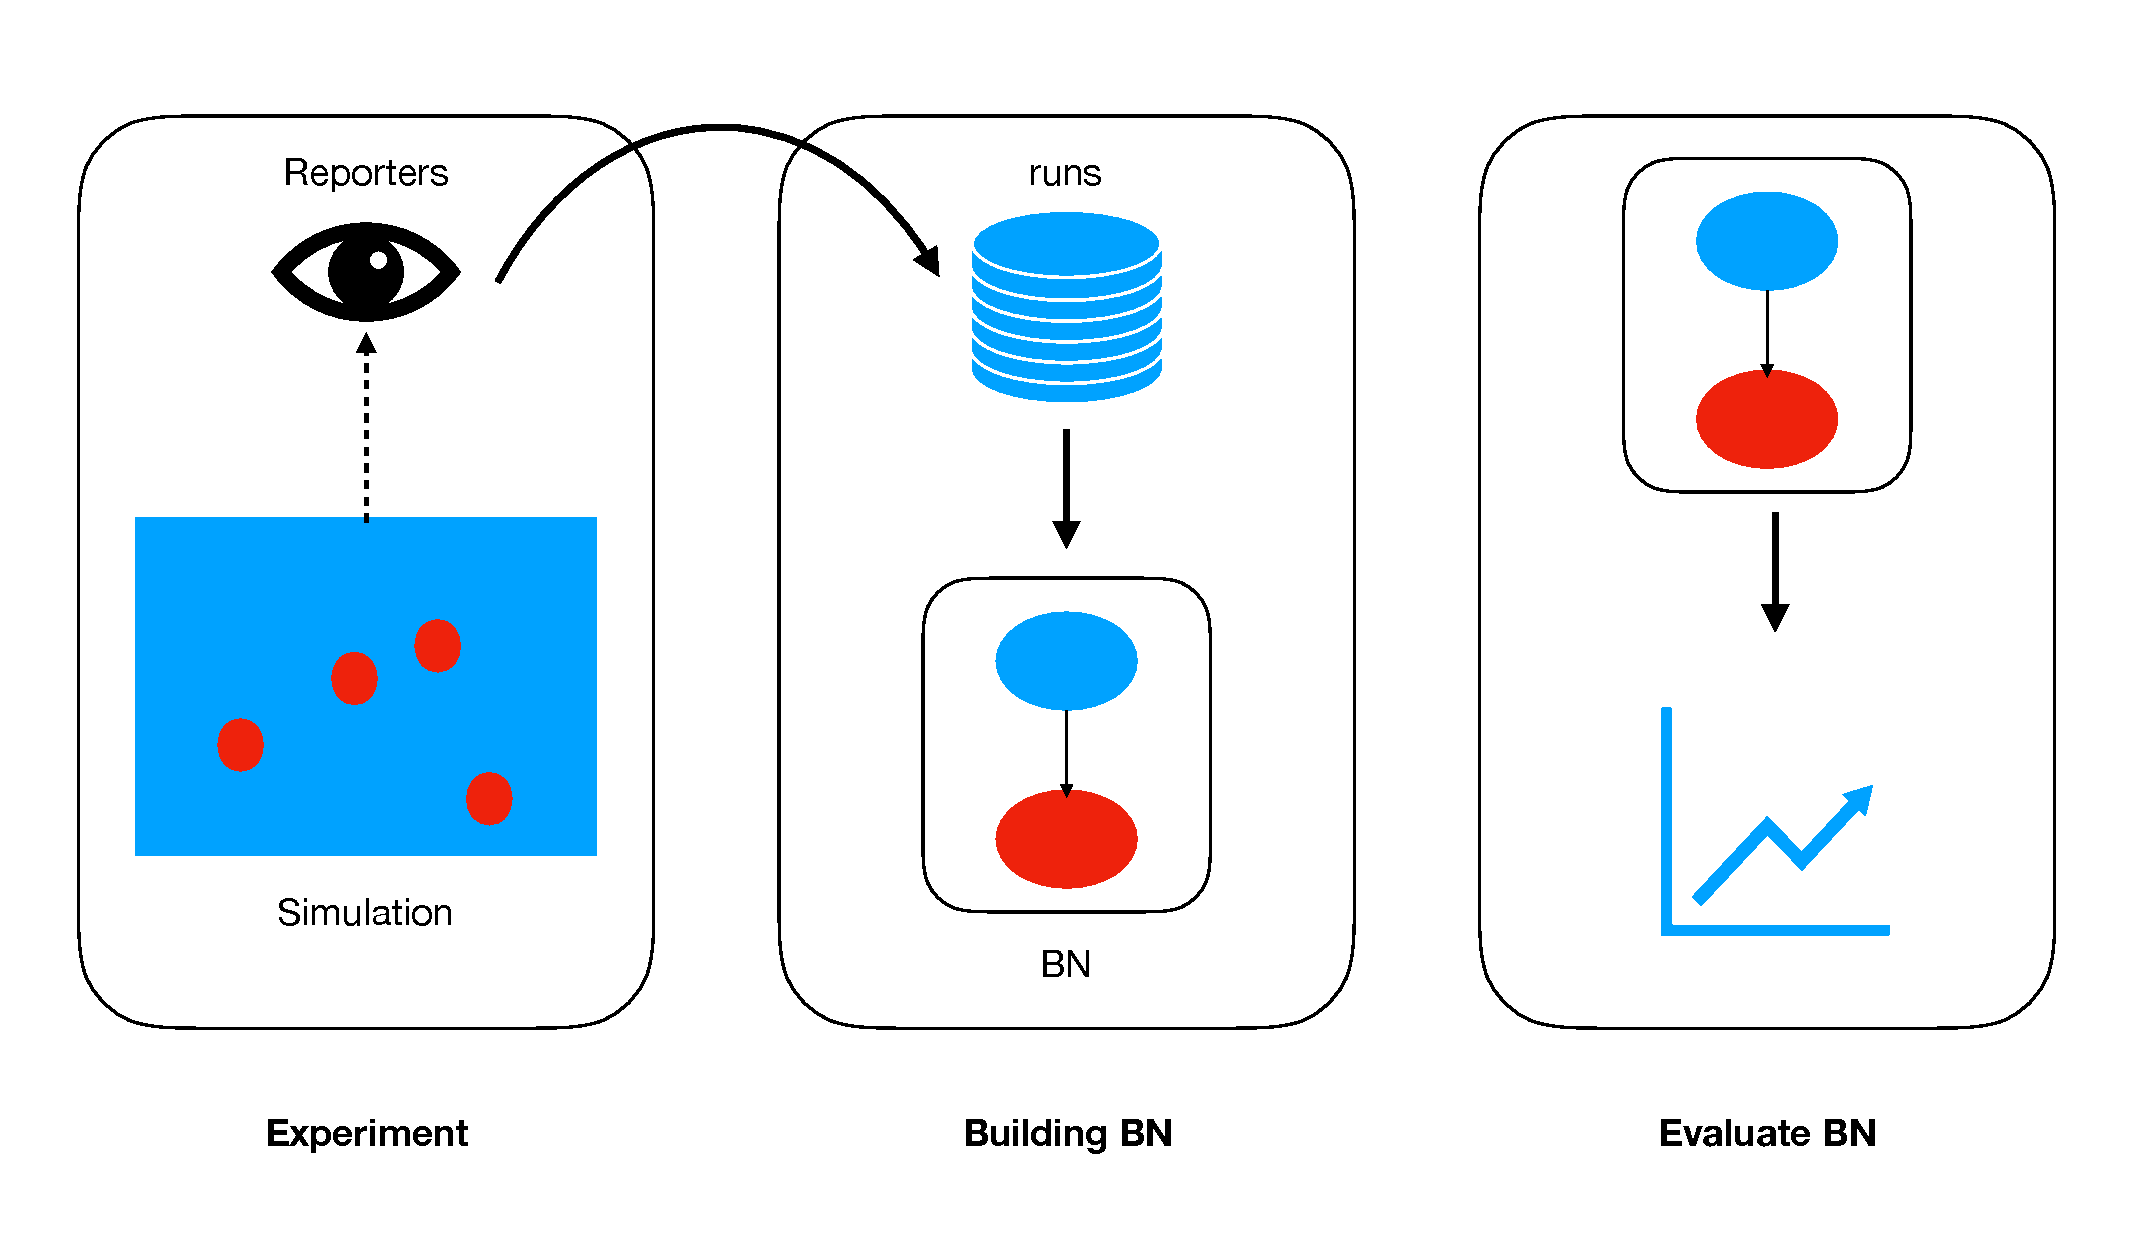
\includegraphics[width=\linewidth]{images/pipeline.pdf}
%\caption{Method for evaluating automatically generated Bayesian Networks from simulations.}
%\label{pipeline}
%\end{figure}

\section{A Scenario}
We start our process with one or more written scenarios. These scenarios can, in the first instance, be obtained from (abridged) court case descriptions. The scenarios should contain all and only those hypothesised events, and the evidence for such events, that are relevant to the case. Both the prosecution and the defence should be able to select relevant events and their evidence. 


\begin{example}
Here we will introduce our running example, loosely based on the first scenario in \citep{Vlek2015}: Mark and Jane live together. One day, a neighbour overhears that they've started to fight in the kitchen. Jane grabs a knife, and stabs Mark. Mark dies of the stab wounds, as confirmed by the forensic scientist at the scene. Jane's fingerprints are on the knife.
\end{example}

\section{An Agent-based Simulation}


We need a way to transform the written text descriptions of the events in the scenario to observable events in the simulation. First we identify all relevant actors, objects and places in the scenario. Then, we divide all all events into three classes: either an event is `evidence', a `hypothesis', or an ultimate `outcome'. The `outcome' is what we are ultimately interested in, it represents the central fact of the case. Apart from it being the node of ultimate interest, it otherwise functions the same as a `hypothesis' node.

Then we select all relevant events from the written description and attempt to operationalise them in the simulation. This means that we create a way to measure if the events take place within the simulation. This is done by means of `reporters', or random variables. These reporters report whether a given event has taken place within the simulation. 

The process of operationalisation is very subjective and depends entirely on the modeller's assumptions and their time, knowledge or skill constraints. The behaviour of agents, as reflections of actual people, can be modelled in a way that reflect real sociological theories of behaviour (such as in \citet{Gerritsen2015}), or with simple rules and a random number generator (such as here). The environment of the simulation can reflect a real-world geography with different affordances, or can be simplified. How a given event is operationalised is essential for the validity of the network: if it is unclear, or disputed, when an event is true in a simulation, the network should not be used.

\begin{example}

We have modelled Jane and Mark as two agents in a simulation (Figure~\ref{tribute}), with as relevant object a knife (blue dot). The only `psychological' aspect that these agents have, is an anger level, which has 4 escalating states = \{not angry, fighting, grabbing knife, stabbing\}. Jane is quicker to increase to the next anger level. 


\begin{figure}[htbp]
\begin{center}
\begin{subfigure}{.5\textwidth}
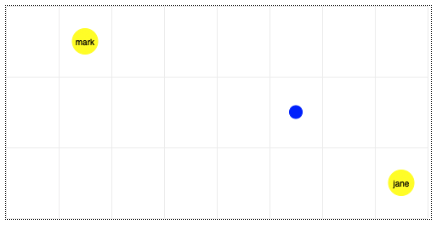
\includegraphics[width=0.9\linewidth]{images/walkthroughSim/s1.png}
\caption{Initial stage of simulation: Mark and Jane are not fighting.}
\label{default}
\end{subfigure}
\begin{subfigure}{.5\textwidth}
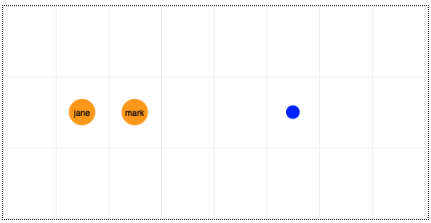
\includegraphics[width=0.9\linewidth]{images/walkthroughSim/s2.png}
\caption{Both Mark and Jane are angry, move towards each other to fight.}
\label{default}
\end{subfigure}
\begin{subfigure}{.5\textwidth}
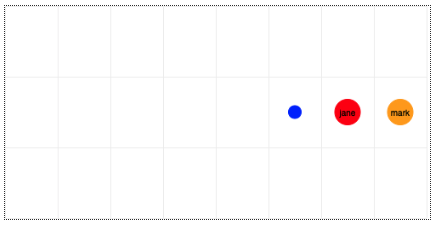
\includegraphics[width=0.9\linewidth]{images/walkthroughSim/s3.png}
\caption{Jane is so angry that she's grabbing the knife.}
\label{default}
\end{subfigure}
\begin{subfigure}{.5\textwidth}
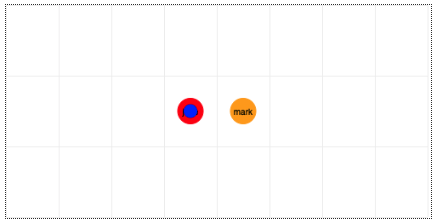
\includegraphics[width=0.9\linewidth]{images/walkthroughSim/s4.png}
\caption{Jane has the knife and moves with it.}
\label{default}
\end{subfigure}
\begin{subfigure}{.5\textwidth}
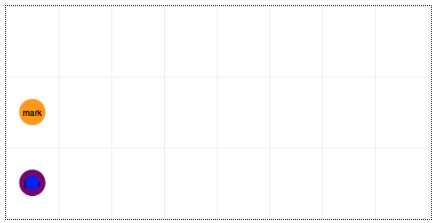
\includegraphics[width=0.9\linewidth]{images/walkthroughSim/s5.png}
\caption{Jane's anger increases by a level, and she stabs Mark.}
\label{default}
\end{subfigure}
\caption{Simulation stages.}
\end{center}
\label{tribute}
\end{figure}


\begin{description}
\item[jane\_and\_mark\_fight ]  Both Mark and Jane have an anger level that is higher than `not angry'
\item[jane\_has\_knife ] Jane has an anger level of `grabbing knife' and moved to the location of the knife
\item[jane\_stabs\_mark\_with\_knife ] Jane has an anger level of `stabbing', has the knife, and moved to Mark's position
\item[mark\_dies ] Jane has stabbed Mark, and if a random number generator (uniform, 0, 100) produces a number $>$ 60
\item[E\_neighbour ] Either Mark and Jane have an anger level that is higher than `not angry'
\item[E\_prints ] True when Jane has knife
\item[E\_stab\_wounds ] True when Jane stabs Mark
\item[E\_forensic ] True when Mark dies

\end{description}

\end{example}




Then, the operationalisation itself: In the simulation, certain events can be brought about. In our example, this could be the events of `jane\_stabs\_mark', or `E\_forensic'.  We need a way to observe these states: this is where reporters come in. A reporter is a random variable that is reports the outcome of a relevant event in the simulation and is embedded in the code. If an event happens (or does not happen), the reporter reports that the event is true (or false). In essence, the reporter ($R$) is a random variable (RV) (for a further explanation of Random Variables, see Chapter 8). In short, a random variable maps an event ($e$) to a truth value:

\[ R : e \rightarrow \{0, 1\} \]

Over which events we define reporters, depends on which events we deem relevant. We could, in theory, create a combinatorial explosive number of reporters for any possible event, like $jane\_in\_position\_(0, 0)$, $jane\_in\_position\_(1, 0)$, etc, but pragmatically, these very granular reporters will not help us in modelling the case. This means that we need to find a balance between over-specification and under-specification.

A reporter's value is 0 by default, but maps an event to 1 whenever it happens in the simulation. When we run the simulation in our example, we expect to see that, whenever Jane and Mark are fighting, $R$ : `jane\_and\_mark\_fight' $\rightarrow 1$. At a later time-step, if Jane stabs Mark, we would see: $R$ : `jane\_stabs\_mark' $\rightarrow 1$.

No matter how many reporters we define, we can combine all reporters at the end of one run of the simulation into a global state $G$.

\[ G = (e_0 \rightarrow \{0, 1\} \times e_1 \rightarrow \{0, 1\} \times ... \times e_n \rightarrow \{0, 1\})\]
 or, for $n$ reporters:
 
\[ G = R_1 \times R_2 \times... \times R_n\]


A global state that would represent that every one of the postulated events and evidence happened, except that Mark did not die of the stabbing, and that there was no forensic scientist to determine that he died of the stab wounds, would be represented as (reporters in the same order as in the listing above):
 \[1,1,1,0,1,1,1,0\]


Then, we collect these global states over the number of runs that we do for each experiment, which results in the output $O$ of this stage of the method, is a series of global states, one for each run:

\[ O = (G_0, G_1, ... G_{runs})\]



\section{Creating a Bayesian Network from a Simulation Automatically}

The output of an experiment is the collection of runs $O$, where each run is the global state $G$ of the simulation, as measured by the random variables $R$. The reporters in the simulation are random variables. These reporters become the nodes in the Bayesian Network.

The Bayesian Network is generated automatically, using the automated BN learner method as implemented in pyAgrum. There are several learners implemented in pyAgrum.\footnote{An introduction to structure learning using PyAgrum: \url{http://webia.lip6.fr/~phw/aGrUM/docs/last/notebooks/structuralLearning.ipynb.html}} The algorithm used in this experiment to structure the Bayesian Network from the simulation data is the K2 algorithm \citep{Cooper1992}. 

The K2 algorithm is a greedy search algorithm that attempts to maximise the posterior probability of the network by correctly connecting parent nodes to child nodes. It takes an ordering on the nodes as input. The first node in the ordering $X_0$ does not have any parents. For two nodes $X_i$ and $X_j$, $X_j$ cannot be the parent node of $X_i$ if $j > i$: a node can only have a parent that is earlier in the ordering. The algorithm processes each node $X_i$ by adding possible parent nodes to $X_i$ (as constrained by the ordering), and maximising the score of the network. The algorithm stops if there are no parents to add, no parents improve the score, or the node has reached the maximal number of parents \citep{Chen2008}.

Due to this ordering constraint, the K2 algorithm is efficient. However, finding the ordering of the nodes as input for the network is not trivial. The ordering should be meaningful, to reflect causal or temporal information present in the domain. Through our simulation, we can find the temporal ordering of the nodes by collecting the temporal order in which hypothesis events occur. The evidence nodes are added at the end, to ensure that evidence nodes are never parents to hypothesis nodes. 

\begin{example}
The temporal ordering of events in the simulation would be:

\{`E\_neighbour', `jane\_and\_mark\_fight', 
`jane\_has\_knife', `E\_prints',
 `jane\_stabs\_mark\_with\_knife', `E\_stab\_wounds',
 `mark\_dies', `E\_forensic' 
 \}
 
 The ordering we want to give to K2 to save the temporal structure and the evidence-idiom \citet{Fenton2012}:
 
 \{ `jane\_and\_mark\_fight', 
`jane\_has\_knife', 
 `jane\_stabs\_mark\_with\_knife', 
 `mark\_dies',
 'E\_neighbour',
  `E\_prints',
 `E\_stab\_wounds',
  `E\_forensic' 
 \}

\end{example}


The ordering is calculated as follows: at every run, we note down which hypothesis events happen in which order. We only note down the order, not the time-step at which an event occurs. We count how often each set of events occurs. We select the set of events that contains the most events, as this is likely the set that represents the entire `causal' chain, or an entire scenario. If there are two sets of events of equal length, we pick the one that occurs most frequently. We add this set first to the ordering. We then look at the number of hypothesis nodes we have left, and add the largest set we can, until we have added all the hypothesis nodes to the ordering. Then we add the evidence nodes to the ordering.

For example, let's say we have 4 hypothesis nodes, $X_1,...X_4$. In Run 1 we find $X_2, X_3, X_4$, in Run 2 we find $X_1$, in Run 3 $X_2, X_3, X_4$ again, but Run 4 is $X_1, X_2, X_3$. We select the longest sets first, and since $X_2, X_3, X_4$ occurs more often than the other one, we add it to the ordering first.  The ordering is now $X_2, X_3, X_4$. We have 4 hypothesis nodes, so we need to add a set of length 1, which is $X_1$, which results in an ordering of $X_2, X_3, X_4, X_1$ that we add evidence to, and apply to the K2 algorithm.


\begin{example}
We give the collection of global states $O$ from our example to K2, as well as the temporal ordering as laid out in the previous example. This results in the a Bayesian Network that is shown in Figure~\ref{genepool}.

\begin{figure}
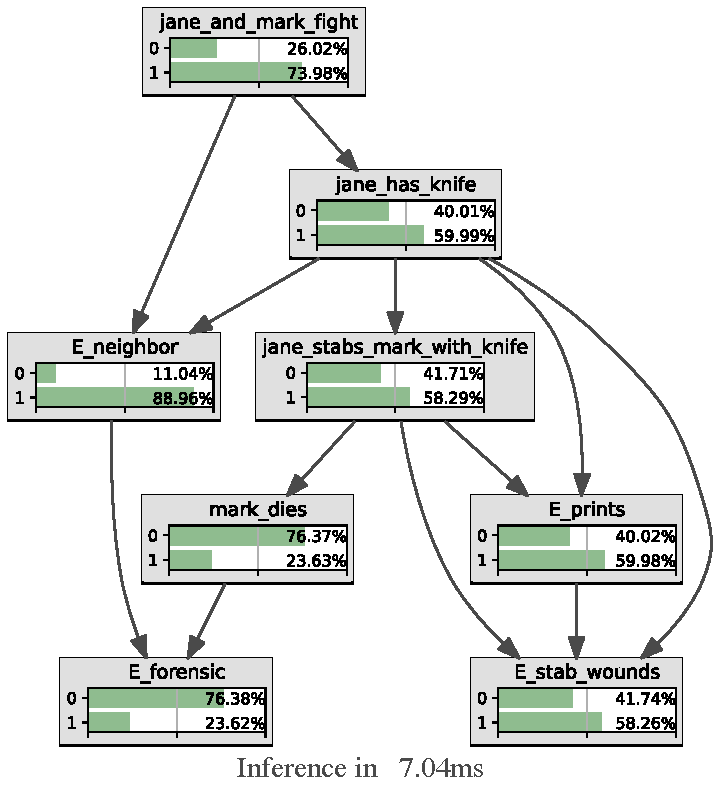
\includegraphics[width=\linewidth]{../experiments/WalkThrough/bnImage/BNIMAGEWalkThrough.pdf}
\caption{Example network.}
\label{genepool}
\end{figure}
\end{example}

After the network is generated, we need to manually change a thing about it. The algorithm does not know how to handle impossible states, which are cases where combinations of valuations for parent nodes are impossible. For example, in Figure~\ref{genepool}, the value of `E\_forensic'. `E\_forensic' has two parents: `mark\_dies', as well as `E\_neighbour'. In the simulation, it can never be the case that Mark dies, but the neighbour does not hear and report on fighting, or the combination of events $`mark\_dies' \rightarrow 1 \land `E\_neighbour' \rightarrow 1$ .  However, the event for the thief stealing the object, can have both `motive' and `knowing about object' as parent nodes. The algorithm does not know how to deal with these situations and the resulting network will crash. This is why the probability for `stealing' given the impossible combination of the parent state values, will be manually set to 0. 


\section{Evaluating the Bayesian Network}

Now we know that we can build Bayesian Networks automatically using the K2 algorithm based on data we generated in our simulation, we need to evaluate different aspects of the Bayesian Network: numerical, structural and performance criteria.


\subsection{Numbers}
\begin{enumerate}
\item \textbf{The conditional frequencies in the BN correspond to the conditional frequencies in the simulation}

We take the collection of global states as the output of the simulation. For every event in the global state, we calculate the base-frequency at which they occur, so if event $A$ occurs 40 times and $\neg A$ occurs 60 times in 100 runs, we find that the frequency of $A = 0.4$. Then, we compare these frequencies with the prior probabilities of the events in the BN.

Given below (Table~\ref{kids}) are the correspondence between the frequencies in the simulation and in the BN. There are differences between the probabilities in the BN and frequencies in the simulation, but these are smaller than $±0.01$.


\begin{table}[htbp]
\centering
\begin{tabular}{|c|c|c|}
 \hline
 Conclusion & Frequency P(event) & BN P(event)\\
 \hline
jane\_and\_mark\_fight & 0.74 & 0.7398 \\
jane\_has\_knife & 0.6 & 0.5999 \\
jane\_stabs\_mark\_with\_knife & 0.583 & 0.5829 \\
mark\_dies & 0.236 & 0.2363 \\
E\_neighbour & 0.89 & 0.8896 \\
E\_prints & 0.6 & 0.5998 \\
E\_stab\_wounds & 0.583 & 0.5826 \\
E\_forensic & 0.236 & 0.2352\\
\hline
\end{tabular}
\caption{Correspondences between simulation frequency and BN}
\label{kids}
\end{table}



\item \textbf{The values in the conditional probability tables are elicitable from human modellers}

In real life, we do not have access to the true frequencies of events in real life. This means that we would have to discover them in some other ways. The CPT in question here, means including the parent node as determined by the K2 algorithm. Relevant questions to ask about the elicitability of CPTs of nodes in the BN are:
\begin{enumerate}
\item Could we discover the frequencies in the CPT using forensic-science methods?
\item Could we discover the frequencies in the CPT using population statistics?
\footnote{Guessing.}
\end{enumerate}

If we have to answer both of these questions with `no', then the CPTs are not elicitable at all. However, answering Question 1 or 2 with a `yes' is not straightforward  - we have to deal with the problem of the reference class.

To show what is meant by that problem, let's apply these questions to our example. We have the node `jane\_has\_knife', given parent node `jane\_and\_mark\_fight', and we want to assign it some probability. However, we cannot find a `population statistic' about `jane\_has\_knife'. Are we going to the CBS and ask about all knife owners named Jane? This is not a meaningful population statistic. Hence, we need to generalise Jane to some class of person that we can find population statistics for. If we generalise `Jane' to the reference class 'a random adult woman in the Netherlands', we could probably find population statistics about knife possession. However, if domestic violence is a pattern in Mark and Jane's relationship (as evidenced by the parent node `jane\_and\_mark\_fight'), we cannot just consider Jane to be `a random adult woman in the Netherlands', but instead consider her `an adult woman in a violent relationship in the Netherlands'. If we find more risk factors and learn more about Jane (high aggression, previous offences, etc.), the subset that we have to find a population statistic over gets smaller and smaller, until we have reached a subjective probability estimation. This is the case for the first question as well.

This problem is unavoidable and it is unclear how we can resolve it. This is a question for future research. However, in this idealised situation, let us always take the most generous interpretation of a node - meaning that we interpret a node as if there might be a reference class. As example, let us divide the nodes into the relevant categories (Table~\ref{cannibal}). 
\begin{table}[htbp]
\centering
\begin{tabular}{|c|c|c|}
 \hline
Node & Forensic science &  Population Statistics \\
 \hline
jane\_and\_mark\_fight &   & x   \\
jane\_has\_knife &   & x  \\
jane\_stabs\_mark\_with\_knife &   & x  \\
mark\_dies &  x &   \\
E\_neighbour &   &   x\\
E\_prints & x  &   \\
E\_stab\_wounds & x  &   \\
E\_forensic & x  &  \\
\hline
\end{tabular}
\caption{Theoretical elicitability}
\label{cannibal}
\end{table}

An important thing to note is that these are \textbf{not} assessments about the actual probability values in the CPTs in the generated BN, but instead only generous theoretical assessments about the deemed possibility of elicitation. The actual probability values in the generated BN will not line up with the forensic or statistical probabilities that we could or would find in real life, since the simulation is very simplified.

\item \textbf{The BN is robust against imprecision in the conditional probability tables}

We can reduce the precision of the values inside the CPTs to investigate the robustness of the BN \citep{Druzdzel2013}. We generate one Bayesian Network, with the data we collected from the simulation. Then, we create many new networks, with this network as a basis. We do not change the number of nodes, nor the structure of the Bayesian network. We only change the values in each node's CPT. In this case, we round the values in the CPT, such that the BN becomes increasingly less precise. The intuition behind this is, that when expert users are going to elicit the probabilities, we do not know how robust the network is against smaller and larger imprecisions in the elicited probabilities. By simulating such imprecisions, we can compare the predictive power of the more imprecise networks to the ground truth of the `real' network. 

We round every value in the cpts $c$ to each of \[i, i \in \{\text{no disturbance}, 0.01, 0.05, 0.1, 0.125, 0.2, 0.25, 0.33, 0.5\} \] according to \[ floor(\frac{c}{i} + 0.5) \cdot i.\]

We also add some imprecision into these networks - so that we never have the values of 0 and 1 in our cpts, as this blocks the propagation of evidence throughout the network. Instead, where we would round to 0 or 1, we round to $1 = \epsilon$ and $\epsilon$, where $\epsilon = 0.01$.

\end{enumerate}

\subsection{Structural}

\begin{enumerate}
\item \textbf{The BN represents all events of the scenario}

We have to define relevance in a meaningful way. The scenario can be split into many different (implicit and explicit) events. The simulation should attempt to model the level of granularity as given in the scenario description, with more detail given in areas where there is conflict between reasoners.

In our example, we modelled every fact as described by the written scenario description. All nodes in the network reflect an event that happened in the scenario. However, the rules that underlie the agent's behaviour (increasing anger, goal-directed movement) are not represented explicitly in the scenario. Using more or less complex behaviour would result in different BNs. Testing different models of criminal behaviour lies outside the scope for this project.

\item \textbf{The BN has temporal ordering of the hypothesis nodes}

We want the BN to follow the temporal structure of the simulation and original scenario. The temporal ordering given to the K2 algorithm should ensure this - however, sometimes there are events that can happen in arbitrary order, or contradict each other with no clear way of determining which events happens first (as they happen exclusively).  

One example of contradictory events, which are not represented in the example network: the simulated `jane\_stabs\_mark\_with\_knife', compared to the non-simulated `mark\_stabbed\_himself'. Apart from the contradictory events or arbitrary temporal events, the hypothesis nodes in the example network are ordered chronologically, in the same order as in the simulation.

\item \textbf{The BN follows the evidence-idiom}

We want to reason from evidence to hypotheses, or, we can observe evidence in real life (or in the simulation), and from there, infer the posterior probability of its parent-hypothesis node. We do not want to do this the other way around, setting a value in a hypothesis node, and looking at the resulting posterior probability of the parent-evidence. This is why evidence must always be the child node of a hypothesis. This construction is also called the evidence idiom \citep{Fenton2012}. Evidence can be the parent of other evidence, as evidence can be dependent on each other \citep{Fenton}.

For example, in the network that was generated for our example, we see that the network fulfils the criterium: There is not a hypothesis node that has an evidence node as a parent.

\item \textbf{The BN represents multiple alternative scenarios}

If we want to model both the scenario as postulated by the defence, and by the prosecution, and let the collective evidence speak, then we need to be able to represent multiple conflicting stories within one BN. Representing different scenarios is not just setting some hypothesis node to false, but instead, it is creating a separate hypothesis node, that contradicts the first node.

 In our example, this would look like, instead of `jane\_stabs\_mark\_with\_knife', the defence would say that `mark\_stabbed\_himself'. These alternative scenarios are not represented in the scenario, simulation or network in this chapter.

\end{enumerate}

\subsection{Predictive}
\begin{enumerate}
\item \textbf{The BN only predicts high probability of the output node given relevant evidence truth values}

We want to use the BN to give a probability estimation of the ultimate output node. We want the probability of the output node to be high if the given evidence supports it, and the probability of this node to be low, when the evidence does not support it. We can test this: given a certain set of evidence, vary the assigned truth values of these evidence nodes, and switch the evidence nodes on in chronological order. We can plot the results, showing a progression of the posterior given a certain set of true or false evidence. Examples of these progression plots are shown in Figure~\ref{internet}.

From these plots, we can see that we can only find a convincing posterior probability for `mark\_dies' when we have the forensic report, the rest of the evidence increases the posterior probability of the node, but never higher than 0.4. This is the expected behaviour - given the operationalisation fo the `E\_forensic' evidence, we expect it (and only it) to weight heavily on the posterior for `mark\_dies'. The other evidence is weaker. 

\begin{figure}[htbp]
\begin{center}
\begin{subfigure}{.66\textwidth}
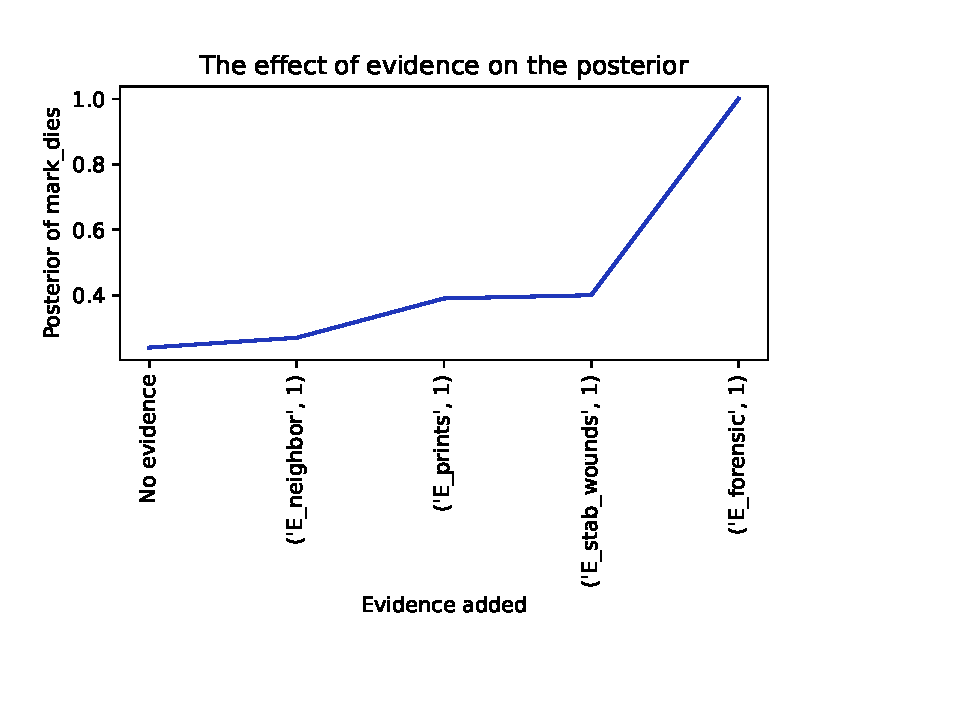
\includegraphics[width=\linewidth]{../experiments/WalkThrough/plots/evidence_progress_WalkThrough_1.pdf}
\caption{All evidence is true.}
\label{default}
\end{subfigure}%
\begin{subfigure}{.66\textwidth}
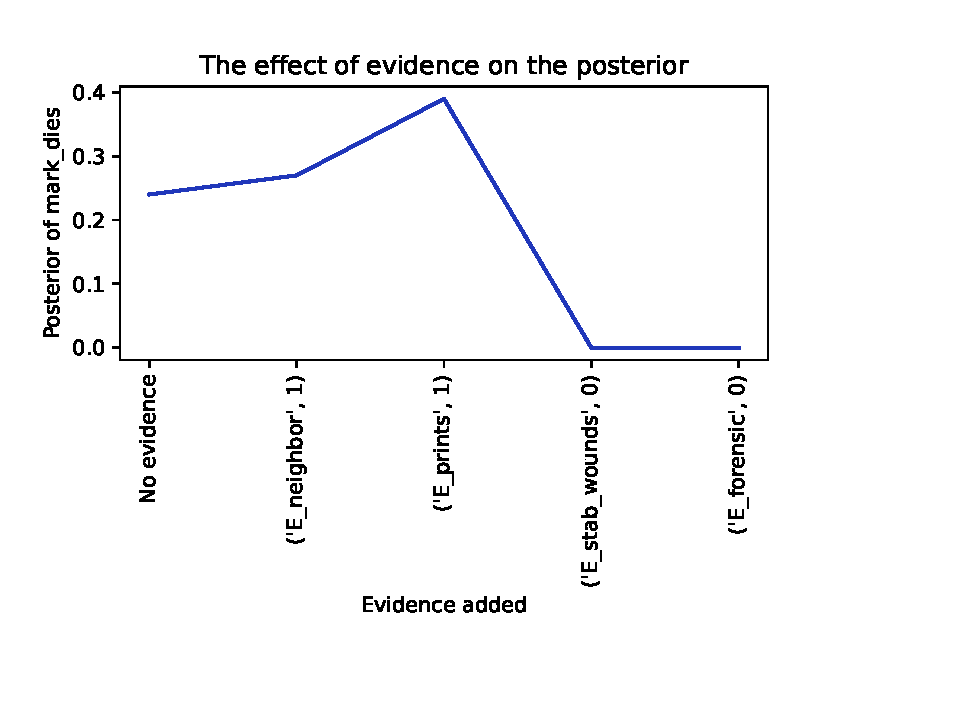
\includegraphics[width=\linewidth]{../experiments/WalkThrough/plots/evidence_progress_WalkThrough_2.pdf}
\caption{Fight, and Jane's prints on the knife.}
\label{default}
\end{subfigure}
\begin{subfigure}{.66\textwidth}
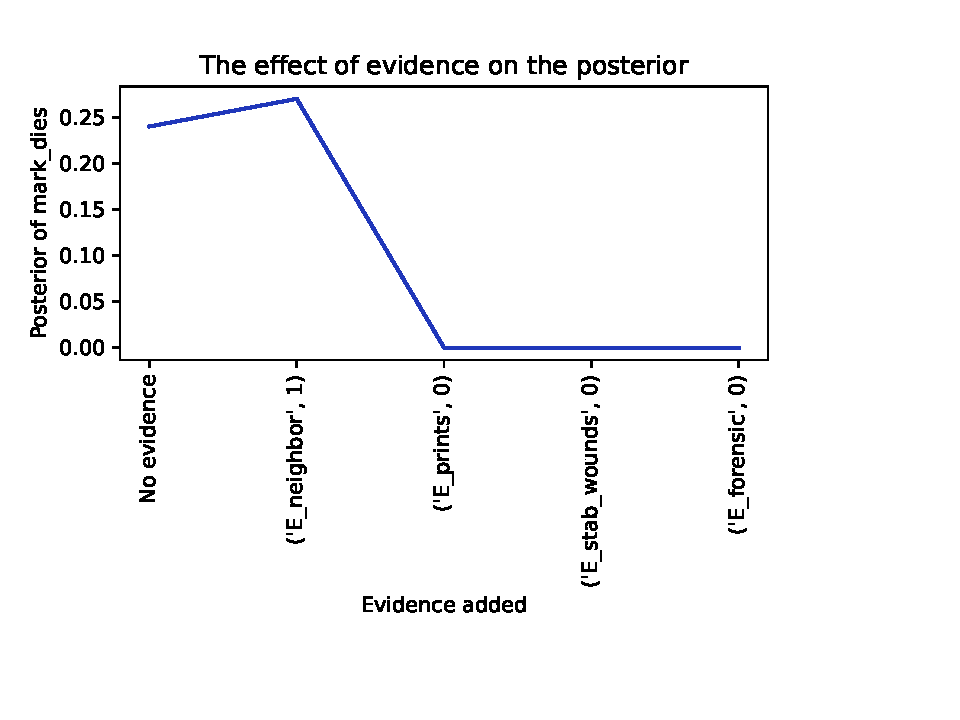
\includegraphics[width=\linewidth]{../experiments/WalkThrough/plots/evidence_progress_WalkThrough_3.pdf}
\caption{Only the neighbour hears them fight.}
\label{default}
\end{subfigure}%
\begin{subfigure}{.66\textwidth}
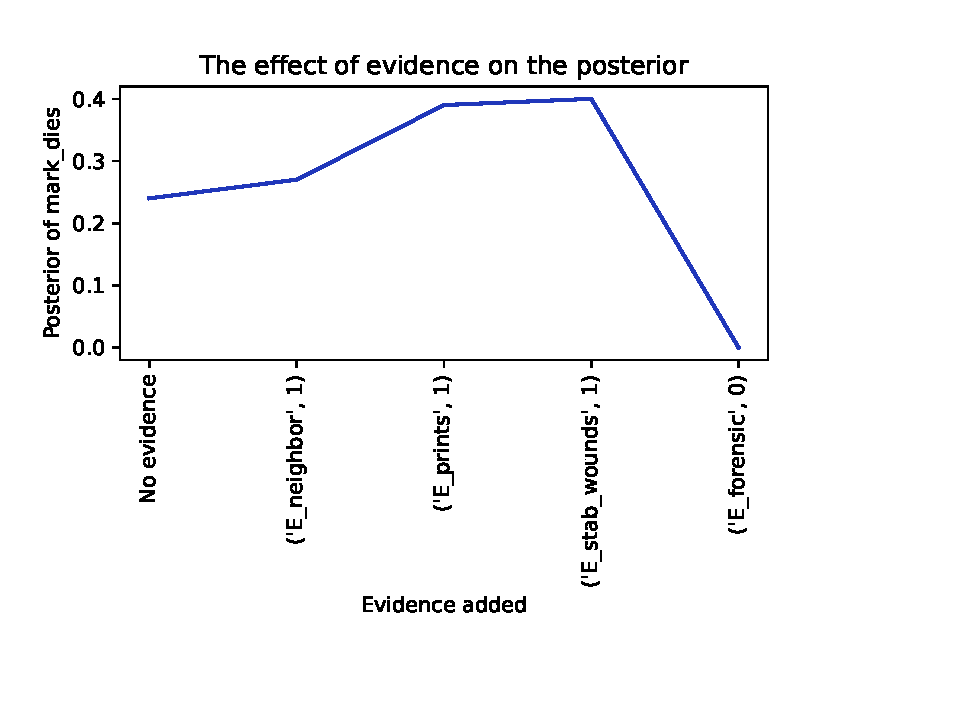
\includegraphics[width=\linewidth]{../experiments/WalkThrough/plots/evidence_progress_WalkThrough_4.pdf}
\caption{Only the death report is false.}
\label{default}
\end{subfigure}
\caption{Effect of evidence on posterior.}
\label{internet}
\end{center}
\end{figure}


\item \textbf{We can know when the BN predicts the wrong outcome}

We investigate all possible permutations of evidence values. There are also impossible permutations of evidence, these are states of evidence that are not allowed by constraints of the simulation, such as the forensic report stating that Mark is dead, but Mark not having stab wounds. These impossible states are not tested. Over the possible evidence states, we show for which evidence states, the network predicts the wrong value for the output node. This means, that in the simulation, given some evidence, the output would happen, but in the BN, given that same set of evidence, the output does not happen. The states for which this occurs are states where the BN is failing. In our example, this is never the case: for all possible evidence states, the network predicts the correct response in the output node.

\end{enumerate}

\section{Conclusion}

In this chapter, we have explained the method for creating and evaluating Bayesian Networks from a simulation based on a written scenario.
